Aliando o poder das RNAs, que reconhecem padrões e se adaptam para lidar com mudanças no ambiente, aos sistemas de inferência \textit{fuzzy}, que incorporam o conhecimento humano e executam inferências e tomadas de decisão, surgiram os sistemas de inferência neuro-\textit{fuzzy} (ANFIS, acrônimo para \textit{Adaptive Neuro-Fuzzy Inference System}), uma nova ferramenta computacional poderosa amplamente utilizada em diversos contextos \cite[p.~1]{Jang1997}.

\subsection{ANFIS: \textit{Adaptive Neuro-Fuzzy Inference Systems}}
Segundo \citeonline[p.~335]{Jang1997}, do ponto de vista funcional, praticamente não há limitações para a gama de funções, no sentido matemático, de uma rede neuro-\textit{fuzzy}, exceto pela exigência de ela ser diferenciável por partes. Devido às mínimas restrições, redes neuro-\textit{fuzzy} podem ser empregadas diretamente em uma grande variedade de aplicações de modelagem, tomadas de decisão, processamento de sinal e controle.

%\subsubsection{Arquitetura ANFIS}
Para simplificar, a arquitetura ANFIS\footnote{Sistema de Inferência Neuro-\textit{Fuzzy} Adaptativo (tradução nossa).} será descrita considerando-a dotada de duas entradas $x$ e $y$ e uma saída $z$. Para um modelo \textit{fuzzy} Sugeno de primeira ordem, um conjunto comum de regras do tipo \textit{se-então} é o seguinte:

\begin{center}
    Regra 1: Se $x$ é $A_1$ e $y$ é $B_1$, então $f_1 = p_1x + q_1y + r_1$,\\
    Regra 2: Se $x$ é $A_2$ e $y$ é $B_2$, então $f_2 = p_2x + q_2y + r_2$. 
\end{center}

A Figura \ref{fig:anfis} ilustra um mecanismo de raciocínio para o modelo Sugeno e a arquitetura ANFIS equivalente, em que nós de uma mesma camada têm funções similares, como descrito a seguir.
\begin{figure}[!htb]
    \centering
    \caption{Equivalência entre modelo \textit{fuzzy} Sugeno e ANFIS; (a) Um modelo \textit{fuzzy} Sugeno com duas entradas de primeira ordem com duas regras; (b) arquitetura ANIFS equivalente}
    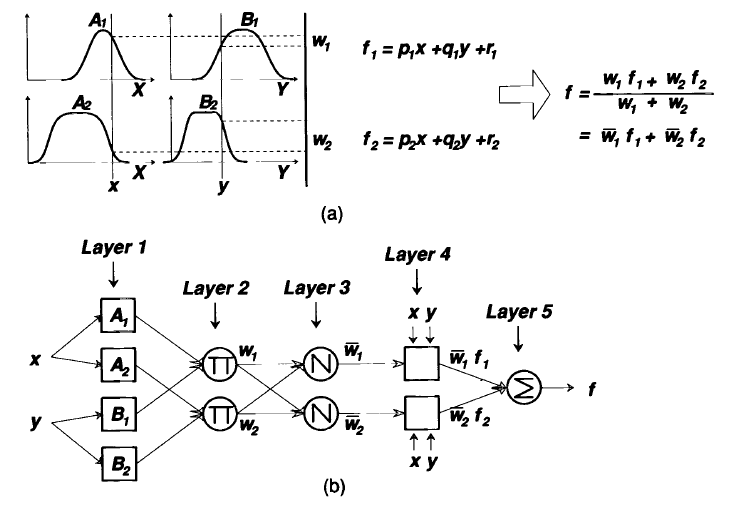
\includegraphics[width=0.8\textwidth]{./04-figuras/fund_teorica/anfis}
    \fonte{\cite[p.~336]{Jang1997}}
    \label{fig:anfis}
\end{figure}

Na camada 1 (\textit{Layer 1}), todo nó \textit{i} é um nó adaptativo com uma função de nó do tipo:
\begin{align*}
    O_{1,i} = \mu_{A_{i}}(x), \mbox{ para } i = 1, 2, \mbox{ ou}\\
    O_{1,i} = \mu_{B_{i-2}}(y), \mbox{ para } i = 3, 4
\end{align*}
em que $x$ (ou $y$) é a entrada para o nó $i$ e $A_{i}$ (ou $B_{i-2}$) é um termo linguístico (como ``pequeno'' ou ``grande'') associado a este nó. Em outras palavras, $O_{1,i}$ é o grau de pertinência de um conjunto \textit{fuzzy} $A$ ($A_1$, $A_2$, $B_1$ ou $B_2$) e especifica o grau em que a entrada $x$ (ou $y$) satisfaz o quantificador $A$. Aqui, a função de pertinência $A$ pode ser qualquer função de pertinência parametrizada apropriada. Parâmetros nesta camada são chamados parâmetros de premissa \cite[p.~336]{Jang1997}.

Na camada 2 (\textit{Layer 2}), cada nó é um nó fixo rotulado $\prod$, cuja saída é o produto de todos sinais de entrada:
\begin{align*}
    O_{2,i} = w_i = \mu_{A_{i}}(x)\mu_{B_{i-2}}(y), i = 1, 2.
\end{align*}

Cada nó de saída representa a força de ativação de uma regra. Em geral, qualquer outro operador norma-T\footnote{Operador de interseção \cite[p.~337]{Jang1997}} que desempenhe a operação \textit{AND} \textit{fuzzy} pode ser usado como função de nó nesta camada \cite[p.~337]{Jang1997}.

Na camada 3 (\textit{Layer 3}), cada nó é um nó fixo rotulado N. O $i$-ésimo nó calcula a taxa da força de ativação da $i$-ésima regra pela soma da força de ativação de todas as regras:
\begin{align*}
    O_{3,i} = \bar{w_i} = \frac{w_i}{w_1 + w_2}, i = 1, 2.
\end{align*}

Por conveniência, saídas desta camada são chamadas forças de ativação normalizadas \cite[p.~336]{Jang1997}.

Na camada 4 (\textit{Layer 4}), todo nó $i$ é um nó adaptativo com uma função nodal
\begin{align*}
    O_{4,i} = \bar{w_i}f_i = \bar{w_i}(p_ix+q_iy+r_i),
\end{align*}
em que $\bar{w_i}$ é um taxa da força de ativação normalizada da camada 3 e \{$p_i, q_i, r_i$\} é o conjunto de parâmetros deste nó. Parâmetros nesta camada são denominados parâmetros consequentes \cite[p.~336]{Jang1997}.

O único nó na camada 5 (\textit{Layer 5}) é um nó fixo denominado $\sum$, e é responsável por computar a saída global como a soma ponderada de todos os sinais de entrada:
\begin{align*}
    \mbox{saída global} = O_{5,i} = \sum_{i} {\bar{w_i}f_i} = \frac{\sum_{i} {w_if_i}}{\sum_{i} {w_i}} %\overline{w_i}(p_ix+q_iy+r_i),
\end{align*}

Com esta arquitetura, constrói-se uma rede neuro-\textit{fuzzy} (ANFIS) que é funcionalmente equivalente a um modelo \textit{fuzzy} Sugeno \cite{Jang1997}. Com isto, sistemas de inferência neuro-\textit{fuzzy} podem operar, por exemplo, utilizando o treinamento supervisionado de uma RNA para ajustar o valor dos parâmetros das funções de resposta dos sistemas de inferência \textit{fuzzy} Sugeno para uma dada operação. Um exemplo de aplicação para este tipo de rede seria o controle de sistemas não lineares.

\subsection{Controladores \textit{Fuzzy} e Neuro-\textit{Fuzzy}}
%Página 451 (Neuro-Fuzzy Control) de Jang1997

Um controlador lógico fuzzy (FLC)\footnote{Do inglês, \textit{Fuzzy Logic Controller}.} é um sistema de inferência fuzzy projetado especificamente para atuar como controlador de um sistema que se deseja controlar. Este FIS portanto possui, como entradas, sinais provenientes do sistema e, como saídas, sinais de atuação sobre ele.

Com o avanço dos microprocessadores e hardware, tem se criado uma diversidade ainda maior de domínios para aplicação de controladores lógicos fuzzy, que vão de eletroeletrônicos à indústria automobilística. De fato, para sistemas complexos ou mal definidos que não são facilmente sujeitados a métodos de controle convencionais, os FLCs proveem uma alternativa viável, uma vez que eles podem capturar os aspectos qualitativos aproximados do raciocínio de um humano e o processo de tomada de decisão. De qualquer forma, sem a capacidade adaptativa, a performance de um FLC se baseia exclusivamente em dois fatores: a disponibilidade de humanos com expertise e as técnicas de aquisição de conhecimento para converter esta expertise humana nas apropriadas regras fuzzy \textit{se-então} e funções de pertinência. Estes dois fatores restringem substancialmente o domínio de aplicações dos FLCs \cite[p.~451]{Jang1997}.

Nesse contexto, o uso de controladores neuro-fuzzy passou a se mostrar muito interessante, tendo em vista que eles eliminam os dois fatores citados que restringem bastante o domínio de aplicações dos FLCs, uma vez que os sistemas ANFIS preenchem as lacunas deixadas pelos FIS, eliminando a necessidade de humanos com expertise sobre o sistema e encorporando técnicas de aquisição de conhecimento.

Com isto, podem-se identificar algumas propriedades particulares aos controladores ANFIS que os tornam ótimas opções para diversos casos \cite[p.~458]{Jang1997}:
\begin{enumerate}
  \item Habilidade de aprendizado;
  \item Operação paralela;
  \item Representação do conhecimento estruturado;
  \item Melhor integração com outros métodos de controle.
\end{enumerate}

Como comparativo, é importante salientar que uma RNA possui as propriedades 1 e 2, mas não as 3 e 4, que são devidas à contribuição dos sistemas de inferência fuzzy \cite[p.~458]{Jang1997}. Um ANFIS, por aliar as duas técnicas, possui todas essas propriedades.

Ainda segundo o autor, há diversas formas diferentes de se projetar controladores neuro-fuzzy. A maioria deles são não lineares. Assim sendo, uma análise rigorosa para sistemas de controle neuro-fuzzy é difícil e continua sendo uma área desafiadora para outras investigações. Por outro lado, um controlador neuro-fuzzy geralmente contém um grande número de parâmetros, o que o torna mais versátil do que um controlador linear ao lidar com características não lineares de plantas. Desta forma, controladores neuro-fuzzy quase sempre superam controladores puramente lineares se devidamente projetados.

%Por outro lado, investigações usando redes neurais em sistemas de controle automatizados não receberam muita atenção até que a regra de aprendizado com \textit{backpropagaion} fosse reformulada em 1986. Desde então, pesquisas de controle neural têm evoluído rapidamente e um grande número de métodos que o implementam tem sido proposto na literatura \cite[p.~451]{Jang1997}.

%\subsubsection{Sistemas de Controle Realimentados}
%A \autoref{fig:feedback-control-system-diagram} é um diagrama de blocos de um típico sistema de controle realimentado, em que a planta (ou processo) representa o sistema dinâmico a ser controlado e o controlador emprega uma estratégia de controle para alcançar um objetivo proposto.
%
%\begin{figure}[!htb]
%    \centering
%    \caption{Diagrama de blocos de um sistema de controle realimentado}
%    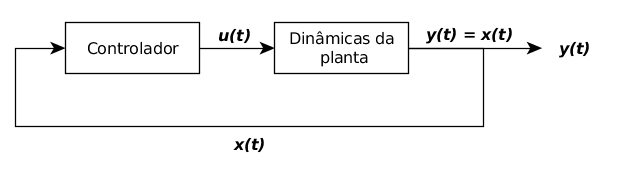
\includegraphics[width=0.9\textwidth]{./04-figuras/Jang1997_feedback_control_system_diagram}
%    \fonte{Adaptado de \citeonline[p.~455]{Jang1997}}
%    \label{fig:feedback-control-system-diagram}
%\end{figure}

%\subsubsection{Controlador Neuro-Fuzzy}
%Se o controlador da \autoref{fig:feedback-control-system-diagram} for substituído por RNAs ou sistemas de inferência fuzzy, obteríamos sistemas de controle neural ou fuzzy, respectivamente. Em outras palavras, métodos de controle neurais ou fuzzy são formas sistemáticas de construir redes neurais ou sistemas de inferência fuzzy como controladores com a intenção de se alcançar um objetivo de controle pré-estabelecido. Da mesma forma, um controle neuro-fuzzy se refere à concepção de métodos para controladores de lógica fuzzy que empregam técnicas de redes neurais. Em particular, podem-se citar métodos para ANFIS \cite[p.~458]{Jang1997}.





%\citeonline[p.~1]{Jang1997} define \textit{Soft Computing}\footnote{Computação Flexível, tradução nossa} (SC) como uma abordagem inovadora para construir sistemas inteligentes computacionais. Segundo ele, chegou-se a um momento em que soluções eficientes para problemas do mundo real requerem sistemas inteligentes que combinem conhecimento, técnicas e metodologias de diferentes fontes. Estes sistemas inteligentes deveriam possuir expertise humanóide com um domínio específico, se adaptar e aprender a agir melhor em mundanças de ambientes e explicar como eles tomam as decisões ou tomam ações.
%
%
%Os diferentes paradigmas que constituem a \textit{Soft Computing} incluem redes neurais, teoria de conjuntos fuzzy, métodos de otimização tais como algoritmos genéticos e \textit{simulated annealing}. Cada um destes métodos possui seu próprio ponto forte, como é mostrado no \autoref{qua:Jang1997_sc_constituents}. A integração adequada destas metodologias formam o núcleo da SC; a sinergia permite à SC a incorporar o conhecimento humano efetivamente, lidar com imprecisão e incerteza, e aprender para se adaptar a diferentes ou desconhecidos ambientes para melhor performance \cite[p.~2]{Jang1997}.
%
%\begin{quadro}[!htb]
    \centering
    \caption{Constituintes da \textit{Soft Computing} e inteligência artificial convencional\label{qua:Jang1997_sc_constituents}}
    \begin{tabular}{|c|c|}
        \hline
            \textbf{Medologia} & 
            \textbf{Ponto Forte} \\
        \hline
            Rede Neural &
            Aprendizado e Adaptção \\
        \hline
            \multirow{2}{*}{Teoria de Conjuntos Fuzzy}&Representação do conhecimento\\
            &via regras se-então\\
        \hline
            Algoritmos Genéticos e \textit{simulated annealing} &
            Pesquisa randômica sistemática \\

        % \hline
        %     \shortstack{Algoritmos Genéticos e \\ \textit{simulated annealing}} &
        %     Pesquisa randômica sistemática\\

        % \hline
        %     \multirow{2}{*}{\shortstack{Algoritmos Genéticos e \\ \textit{simulated annealing}}} &
        %     Pesquisa randômica sistemática\\

        \hline
            IA Convencional &
            Manipulação Simbólica \\
        \hline
    \end{tabular}
    \fonte{Adaptado de \citeonline[p.~2]{Jang1997}}
\end{quadro}
